%This is the first chapter of the dissertation

%The following command starts your chapter. If you want different titles used in your ToC and at the top of the page throughout the chapter, you can specify those values here. Since Columbia doesn't want extra information in the headers and footers, the "Top of Page Title" value won't actually appear.

\chapter[The Large Hadron Collider][Top of Page Title]{The Large Hadron Collider}

The Large Hadron Collider (LHC) produces high-energy protons which are collided at the center of multiple large experiments at CERN on the outskirts of Geneva, Switzerland \cite{Evans:2008zzb}.
The LHC produces the highest energy collisions in the world, with design center-of-mass energy of $\sqrt{s} = 14 \GeV$, which allows the experiments to investigate physics far beyond the reach of previous colliders \todo{cite fermilab?}
This brief chapter will summarize the very basics of accelerator physics.
We will describe the CERN accelerator complex and the LHC.

\section{Basics of Accelerator Physics}

This section follows closely the presentation of \cite{ShiltsevColliderLectures}.

Simple particle accelerators simply rely on the acceleration of charged particles in a static electric field.
Given a field of strength $E$, charge $q$, and mass $m$, this is simply
\begin{equation}
a = \frac{qE}{m}.
\end{equation}
This was used for many early accelerators \todo{cite some?}
For a given particle with a given mass and charge, this is of course limited by the static electric field which can be produced.
This is limited by the electric breakdown at high voltages.

There are two complementary solutions to this issue.
First, we use the \textit{radio frequency acceleration} technique.
This consist of using a time-varied electric field.
We call the devices used for this \textit{RF cavities}.
Second, one bends the particles in a magnetic field, which allows them to pass through the same RF electric field over and over.
This second process is limited by \textit{synchrotron radiation}, which describes the radiation produced when a charged particle is accelerated.
The power radiated is
\begin{equation}
P \order \frac{1}{r^2} \begin{pmatrix} E/m \end{pmatrix}^4
\end{equation}
where $r$ is the radius of curvature and $E,m$ is the energy (mass) of the charged particle.
Given an energy which can be produced by a given set of RF cavities (which is \textit{not} limited by the mass of the particle), one then has two options to increase the actual collision energy : increase the radius of curvature or use a heavier particle.
Practically speaking, the easiest options for particles in a collider are protons and electrons, since they are (obviously) copious in nature and do not decay\footnotemark.
\footnotetext{Muon colliders are a really cool option at high energies, since the relativistic $\gamma$ factor gives them a relatively long lifetime in the lab frame.}
Given the dependence on mass, we can see why protons are used to reach the highest energies.
The tradeoff for this is that protons are not point particles, and we thus we don't know the exact incoming four-vectors of the protons, as discussed in Ch.\ref{ch:sm}.

The primary ``unit'' of a proton-proton collider is the (proton) \textit{bunch}.
All of the bunches together are called the \textit{beam}.
An important property of a beam of a particular energy $E$, moving in uniform magnetic field $B$, containing particles of momentum p is the \textit{beam rigidity} :
\begin{equation}\label{eq:rigidity}
R \equiv r B = p / c.
\end{equation}
The linear relation between $r$ and $p$, or alternatively $B$ and $p$ have important consequences for LHC physics.

Bunches of protons are induced by the RF cavities; particles are accelerated or deccelerated by the cavities, and pushed together into bunches, which eventually pass through the RF cavities at the frequency of the cavity.
Besides the rigidity of the beam, the most important quantities to characterize a beam are known as the (normalized) \textit{emittance} $\epsilon_N$ and the \textit{betatron function} $\beta$.\todo{cite betatron function} \todo{add fig of emittance}.
These quantities determine the transverse size $\sigma$ of a relativistic beam $v <\order c$ beam : $\sigma^2 = \beta^* \epsilon_N / \gamma_{\text{rel}}$, where $\beta^*$ is the value of the betatron function at the collision point and $\gamma_{\text{rel}}$ is the standard relativistic $\gamma$ value.

These quantities determine the \textit{instaneous luminosity} of a collider, which combined with the cross-section $\sigma$ of a particular physics process, give the rate of this physics process.
For process of cross-section $\sigma$, the rate is given by
\begin{equation} \ref{eq:rate}
R = L \sigma
\end{equation}
where $L$ is the instaneous luminosity, given by:
\begin{equation}\ref{eq:insta_lumi}
L = \frac{f_{\text{rev}} N_b^2 F}{4 \pi \sigma^2}= \frac{f_{\text{rev}} n N_b^2 \gamma_{\text{rel}} F }{ 4\pi \beta^* \epsilon_N}.
\end{equation}
Here we have introduced the frequency of revolutions $f_{\text{rev}}$, the number of bunches $n$, the number of protons per bunch $N_b^2$, and a geometric factor $F$ related to the crossing angle of the beams.

The \textit{integrated luminosity} $\int_{}^{} L$ gives the total number of a particular physics process $P$, with cross-section $\sigma_{\text{P}}$.
\begin{equation}
N_{\text{P}} = \sigma_{\text{P}} \int_{}^{} L.
\end{equation}
Due to this simple relation, one can also quantify the ``amount of data delivered'' by a collider simply by $\int_{}^{} L$.

\section{Accelerator Complex}

The Large Hadron Collider is the last accelerator in a chain of accelerators which together form the CERN accelerator complex, which can be seen in \ref{fig:accelerator_complex}.
\begin{figure}
\caption{The CERN accelerator complex.}\label{fig:accelerator_complex}
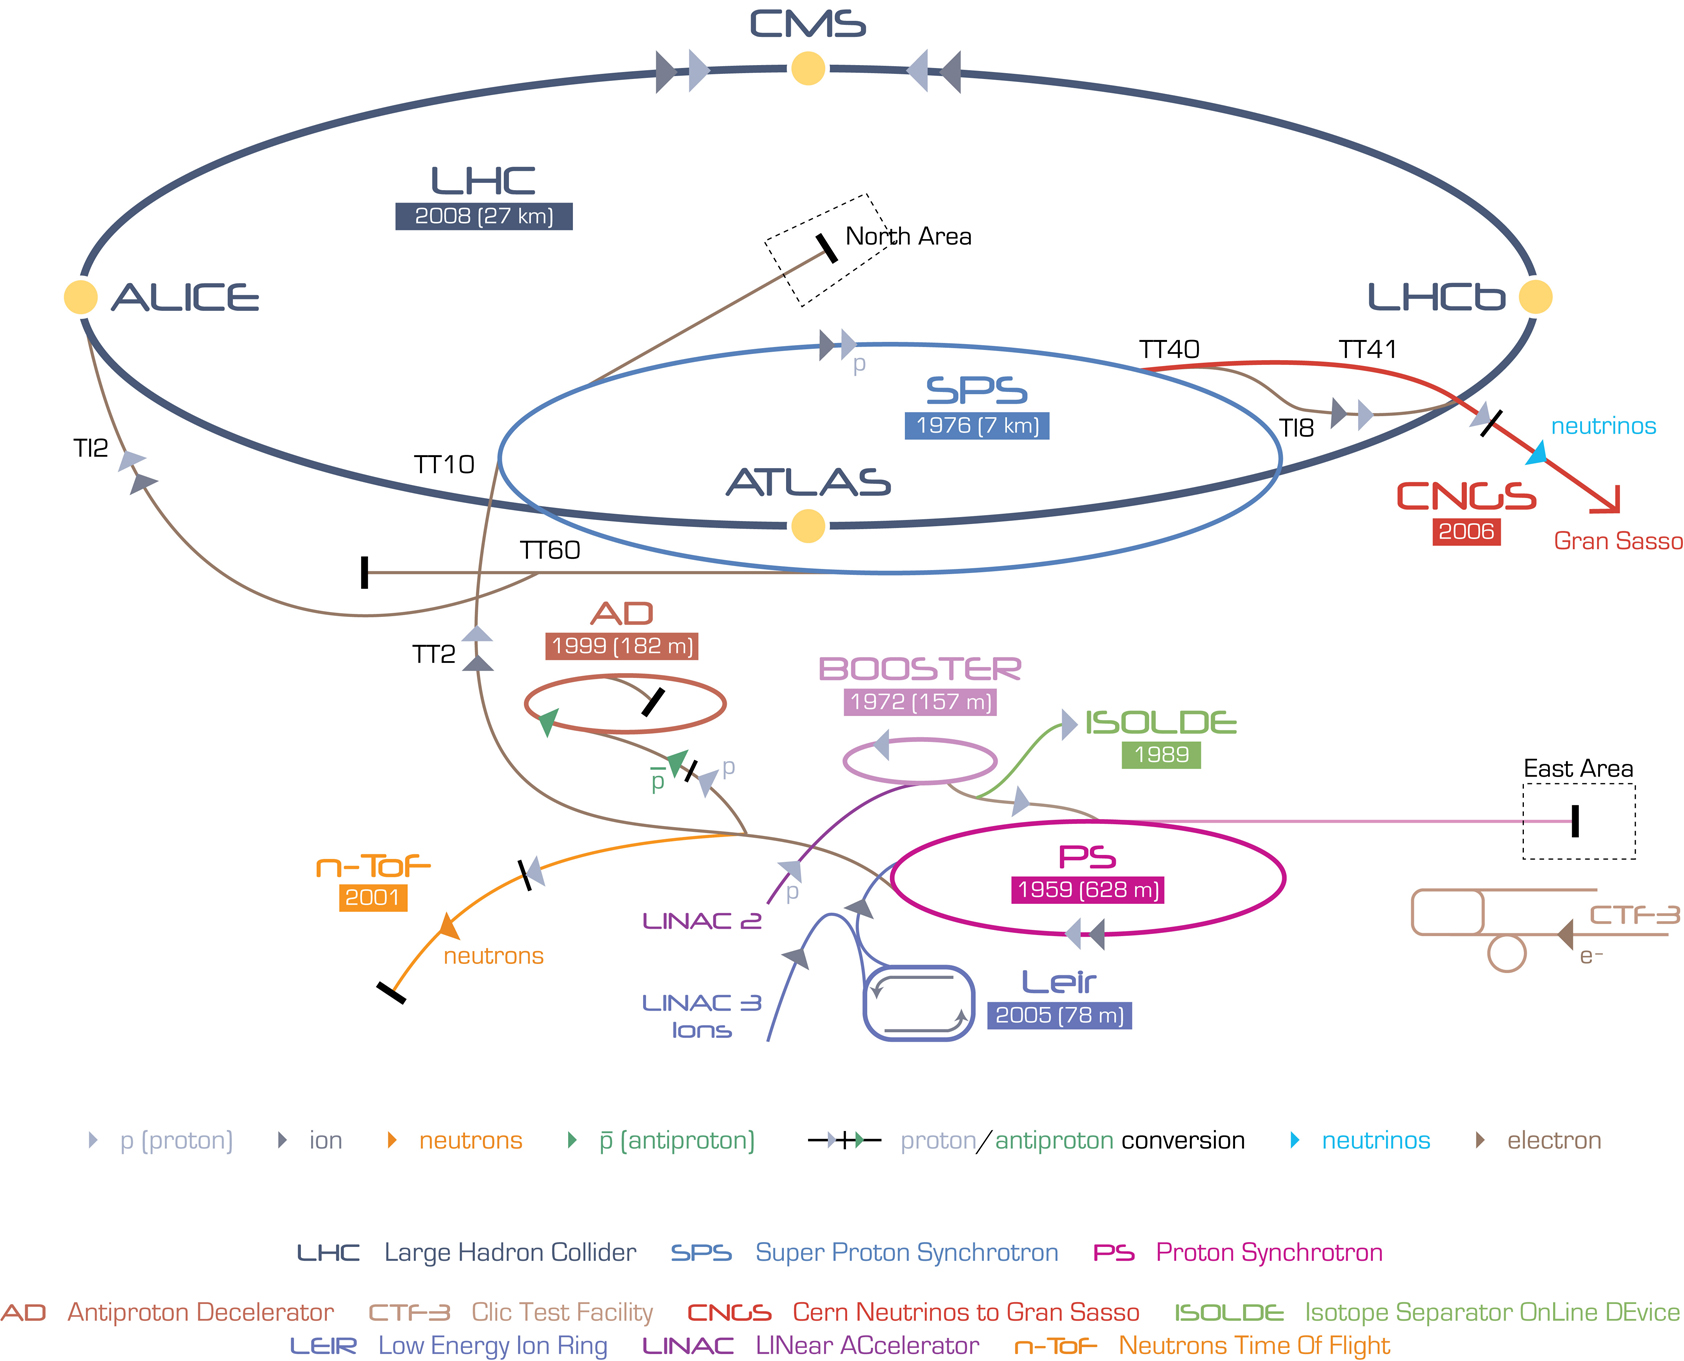
\includegraphics[width=.9\linewidth]{Cern-Accelerator-Complex}
\end{figure}
The protons begin their journey to annilation in a hydrogen source, where they are subsequently ionized.
The first acceleration occurs in the Linac 2, a linear accelerator composed of RF cavities.
The protons leave the Linac 2 at an energy of $50 \MeV$ and enter the Proton Synchrotron Booster (PSB).
The PSB contains four superimposed rings, which accelerate the protons to $1.4 \GeV$.
The protons are then injected into the Proton Synchrotron (PS).
This synchrotron increases the energy up to 25 GeV.
After leaving the PS, the protons enter the Super Proton Synchrotron (SPS).
This is the last step before entering the LHC ring, and the protons are accelerated to $450 \GeV$.
From the SPS, the protons are injected into the beam pipes of the LHC.
The process to fill the LHC rings with proton bunches from start to finish typically takes about four minutes.

\section{Large Hadron Collider}

The Large Hadron Collider is the final step in the CERN accelerator complex, and produces the collisions analyzed in this thesis.
From the point of view of experimentalists on the general-purpose ATLAS and CMS experiments, the main goal of the LHC is to deliver collisions at the highest possible energy, with the highest possible instaneous luminosity.
The LHC was installed in the existing 27 km tunnel used by the Large Electron Positron (LEP) collider.\todo{cite}
This allowed the existing accelerator complex at CERN, described in the previous section, to be used as the injection system to prepare the protons up to $450 \GeV$.
Many aspects of the LHC design were decided by this very fact, and specified the options allowed to increase the energy or luminosity.
In particular, the radius of the tunnel was already specified; from Eq.\ref{eq:rigidity}, this implies the momentum (or energy) of the beam is entirely determined by the magnetic field.
Given the 27 km circumference of the LEP tunnel, one can calculate the required magnetic field to reach the 7 \TeV per proton design energy of the LHC :
\begin{align}
r &= C / 2\pi = 4.3 km \\
\rightarrow B &= \frac{p}{rc} = 5 T
\end{align}
In fact, the LHC consists of 8 528 m straight portions consisting of RF cavities, used to accelerate the particles, and 8 circular portions which bend the protons around the LHC ring.
The circular portions actually have a slightly smaller radius of curvature $r = 2804 $ m, and we require $B = 8.33 T$.
To produce this large field, we need to use superconducting magnets, as discussed in the next section.

\subsection{Magnets}

There are many magnets used by the LHC machine, but the most important are the 1232 dipole magnets; a schematic is shown in Fig.\ref{fig:dipole_schematic} and a photograph is shown in Fig.\ref{fig:dipole_photo}.
\begin{figure}
\caption{Schematic of an LHC dipole magnet.}\label{fig:dipole_schematic}
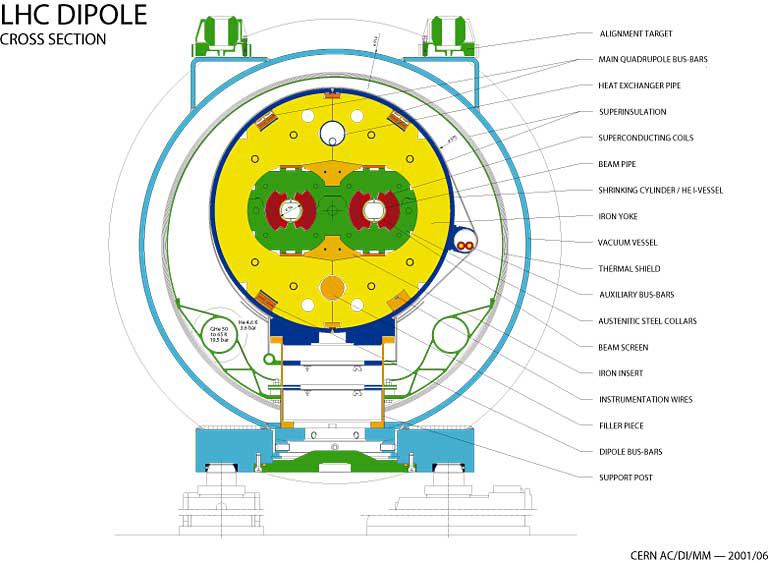
\includegraphics[width=.9\linewidth]{lhc_dipole}
\end{figure}

\begin{figure}
\caption{Photograph of a technician connecting an LHC dipole magnet.}\label{fig:dipole_photo}
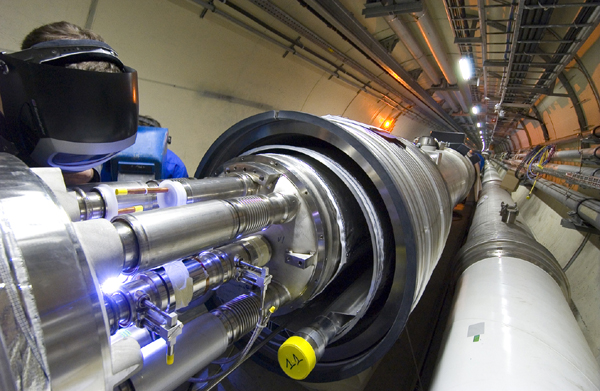
\includegraphics[width=.9\linewidth]{dipole_photo}
\end{figure}
The magnets are made of Niobium and Titanium.
The maximum field strength is 10 T when cooled to 1.9 Kelvin.
The magnets are cooled by superfluid helium, which is supplied by a large cryogenic system.
Due to heating between the eight helium refrigerators and the beampipe, the helium is cooled in the refrigerators to 1.8 K.

A failure in the cooling system can cause what is known as a \textit{quench}.
If the temperature goes above the critical superconducting temperature, the metal loses its superconducting properties, which leads to a large resistance in the metal.
This leads to rapid temperature increases (following $P_{\text{rad}} = I^2 R$), and can cause extensive damages if not controlled.

The dipole magnets are 16.5 meters long with a diameter of 0.57 meters.
There are two individual beam pipes inside each magnet, which allows the dipoles to house the beams travelling in both directions around the LHC ring.
They curve slightly, at an angle of 5.1 mrad, which carefully matches the curvature of the ring.
The beampipes inside of the magnets are held in high vacuum, to avoid stray particles interacting with the beam.

The beam parameters relevant to the dataset analyzed in this thesis are available in Table \ref{tab:lhc_beam_parameters}.
\begin{table}
\centering
\caption{Beam parameters of the Large Hadron Collider.}\label{tab:lhc_beam_parameters}
\begin{tabular}{| l | l | l |}
\hline
Parameter  & Injection & Extraction                           \\ \hhline{|=|=|=|}
Energy (\GeV)    & 450   & 7000  \\ \hline
Rigidity (T-m)   & 3.8   & 23353 \\ \hline
Bunch spacing (ns) & 25 & 25 \\ \hline
Design Luminosity ($\text{cm}^{-2} \text{s}^{-1} \times 10^34$) & - & 1.0 \\ \hline
Bunches per proton beam & 2808 & 2808\\ \hline
Protons per bunch       & 1.15 e11 & 1.15 e11 \\ \hline
Beam lifetime (hr)      & - & 10 \\ \hline
Normalized Emittance $\epsilon_N$ (mm $\mu$rad) & 3.3 & 3.75 \\ \hline
Betatron function at collision point $\beta^*$ (cm) & - & 55 \\ \hline
\end{tabular}
\end{table}

\section{Dataset Delivered by the LHC}

In this thesis, we analyze the data delivered by the LHC to ATLAS in the 2015 and 2016 datasets.
The peak instaneous luminosity delivered in 2015 (2016) was $L = 5.2 (11) \text{cm}^{-2} \text{s}^{-1} \times 10^33 $.
One can note that the instaneous luminosity delivered in the 2016 dataset exceeds the design luminosity of the LHC.
The total integrated luminosity delivered was 13.3 \ifb.
One can see the integrated luminosity as a function of day for 2015 and 2016 in Figure \ref{fig:lumi}\footnotemark
\footnotetext{This thesis analyzes results through ICHEP2016.
The corresponding 2016 plot for the year to date can be found at the ATLAS lumonosity group \href{https://twiki.cern.ch/twiki/bin/view/AtlasPublic/LuminosityPublicResultsRun2}{twiki}.}
\begin{figure}
\caption{Photograph of a technician connecting an LHC dipole magnet.}\label{fig}
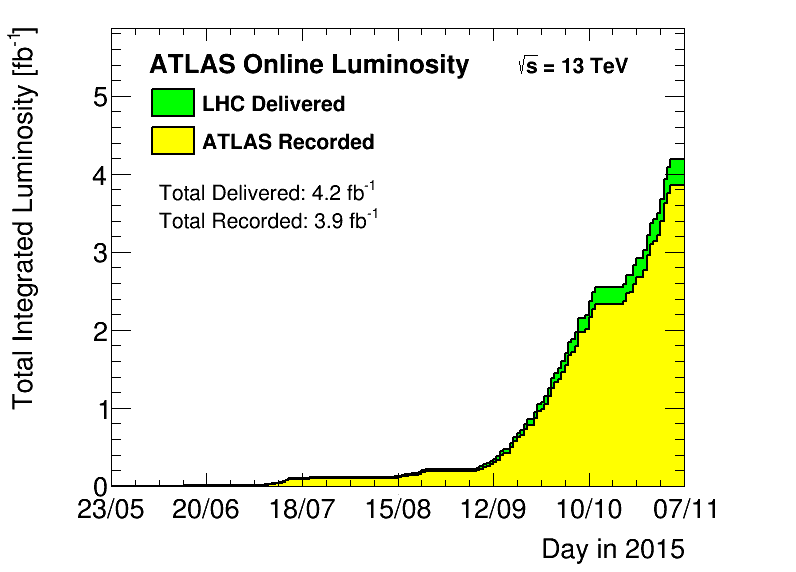
\includegraphics[width=.9\linewidth]{lumi_2015}
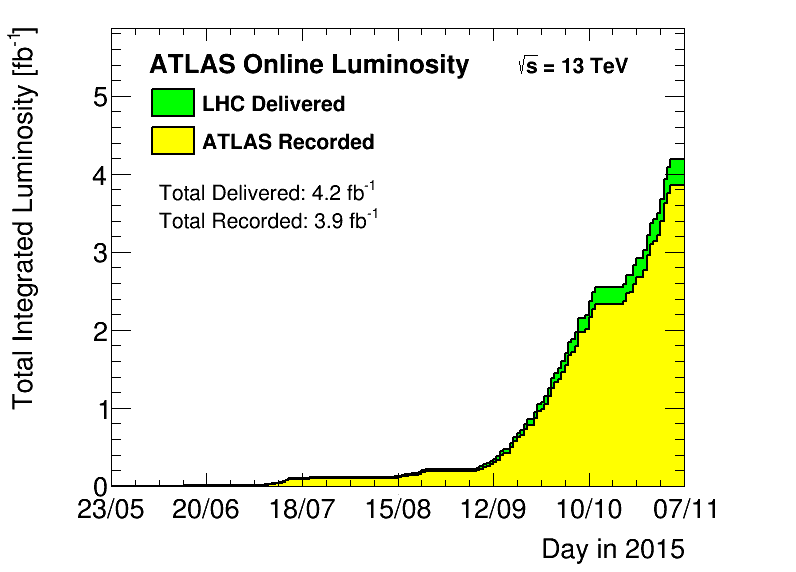
\includegraphics[width=.9\linewidth]{lumi_2015}
\end{figure}
We also see the ATLAS distinction of ``All Good for Physics'', which will be described in the next chapter.
Here we suffice to state that there are additional requirements placed on the detector operation to ensure quality measurements.

\subsection{Pileup}

\textit{Pileup} is the term for the additional proton-proton interactions which occur during each bunch crossing at the center of the ATLAS detector.
At the beginning of the LHC physics program, there had not been a collider which averaged more than a single interaction per bunch crossing.
In the LHC, each bunch crossing (or \textit{event})  generally contains multiple proton-proton interactions.
An example event with many \textit{vertices} can be seen in Fig.\ref{fig:pileup_reconstruction}
\begin{figure}
\caption{Photograph of a technician connecting an LHC dipole magnet.}\label{fig:pileup_reconstruction}
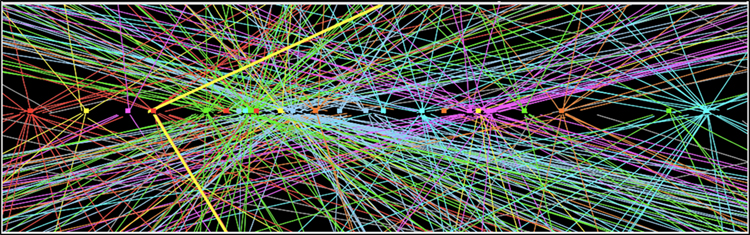
\includegraphics[width=.9\linewidth]{pileup_reconstruction}
\end{figure}
The so-called \textit{primary vertex} (or \textit{hard scatter vertex}) refers to the vertex which has the highest $\Sigma p_T^2$;  this summation occurs over the \textit{tracks} in the detector, which we will describe later.
We then distinguish between \textit{in-time} pileup and \textit{out-of-time} pileup.
In-time pileup refers to the additional proton-proton interactions which occur in the event.
Out-of-time pileup refers to effects related to proton-proton interactions previous bunch crossings.

We quantify in-time pileup by the number of ``primary''\footnotemark vertices in a particular event.
\footnotetext{\textit{The} primary vertex is as defined above, but we unfortunately use the same name here.}
To quantify the out-of-time pileup, we use the average number of interactions per bunch crossing $<\mu>$ over some human-scale time.
In Figure \ref{fig:pileup}, we show the distribution of $\mu$ for the dataset used in this thesis\todo{2016!!!!}.
\begin{figure}
\caption{Photograph of a technician connecting an LHC dipole magnet.}\label{fig:pileup}
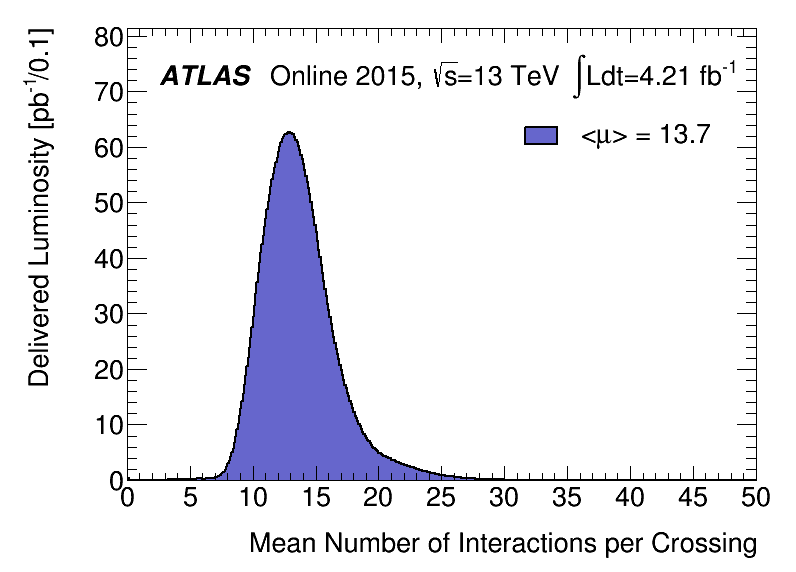
\includegraphics[width=.9\linewidth]{pileup_2015}
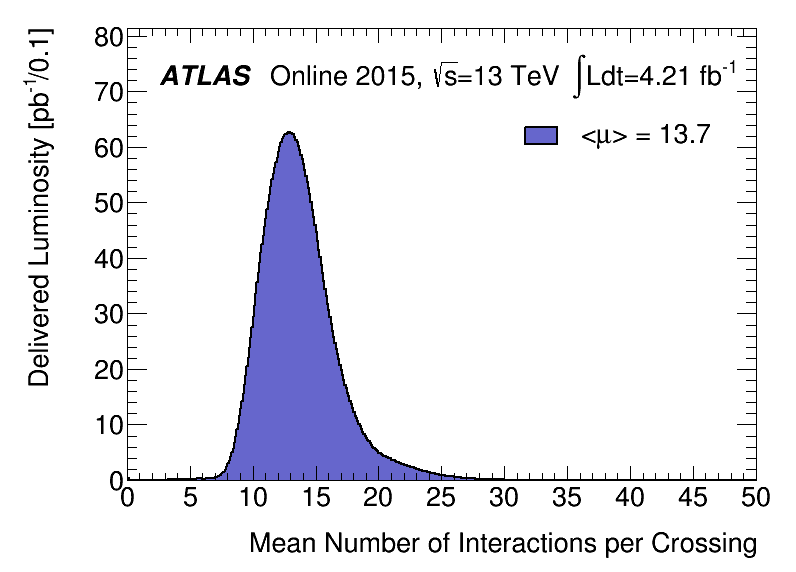
\includegraphics[width=.9\linewidth]{pileup_2015}
\end{figure}
